\documentclass{beamer}
\usetheme{Hannover}
\setbeamersize{sidebar width left=0pt}
\usepackage[T1, T2A]{fontenc}
\usepackage[utf8]{inputenc}
\usepackage[russian]{babel}
\usepackage{hyperref}
\usepackage{graphicx}
\graphicspath{ {../Images/} }

\author{Григорий Матюхин}
\date{\today}
\title{Лабораторная работа \textnumero6.}
\subtitle{Управление процессами}

\begin{document}
\begin{frame}[plain]
	\titlepage
\end{frame}
\section{Цель работы}
\begin{frame}[plain]
	\frametitle{Цель работы}
	Получить навыки управления процессами операционной системы.
\end{frame}

\section{Последовательность выполнения работы}
\subsection{Управление заданиями}
\begin{enumerate}
	\begin{frame}[plain]
		\frametitle{Управление заданиями}
		\item Введите следующие команды: \\
		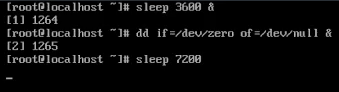
\includegraphics{1.png}
		\item Поскольку вы запустили последнюю команду без \& после неё, у вас есть 2 часа,прежде чем вы снова получите контроль над оболочкой. Введите Ctrl + z , чтобы остановить процесс: \\
		
\includegraphics{2.png}
	\end{frame}
	\begin{frame}[plain]
		\item Посмторите текущие задания: \\
		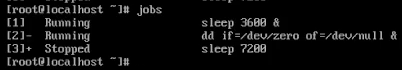
\includegraphics{3.png}
		\item Для продолжения выполнения задания 3 в фоновом режиме введите bg 3. С помощью команды jobs посмотрите изменения в статусе заданий. \\
		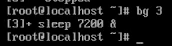
\includegraphics{4.png}
	\end{frame}
	\begin{frame}[plain]
		\item Для перемещения задания 1 на передний план введите fg 1: \\
		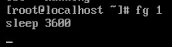
\includegraphics{5.png}
		\item Введите Ctrl + c , чтобы отменить задание 1. С помощью команды jobs посмотрите изменения в статусе заданий: \\
		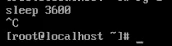
\includegraphics{6.png}
	\end{frame}
	\begin{frame}[plain]
		\item Проделайте то же самое для отмены заданий 2 и 3: \\
		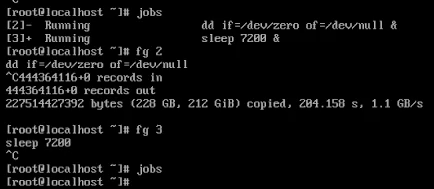
\includegraphics{7.png}
	\end{frame}
	\begin{frame}[plain]
		\item Откройте второй терминал и под учётной записью своего пользователя и запустите в нём \texttt{dd if=/dev/zero of=/dev/null \&}:
		\item Введите exit, чтобы закрыть второй терминал: \\
		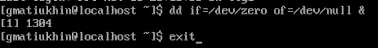
\includegraphics{8.png}
	\end{frame}
	\begin{frame}[plain]
		\item На другом терминале под учётной записью своего пользователя запустите top: \\
		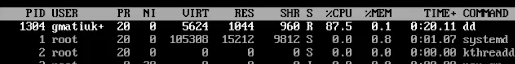
\includegraphics{9.png}
		\item Вновь запустите top и в нём используйте k , чтобы убить задание dd. После этого выйдите из top: \\
		
\includegraphics{10.png}
	\end{frame}
\end{enumerate}

\subsection{Управление процессами}
\begin{enumerate}
	\begin{frame}[plain]
		\frametitle{Управление процессами}
		\item Посмотрите запущенные процессы: \\
		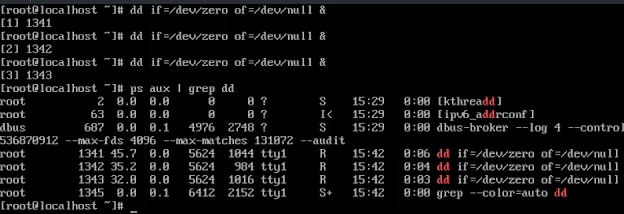
\includegraphics{11.png}
	\end{frame}
	\begin{frame}[plain]
		\item Используйте PID одного из процессов dd, чтобы изменить приоритет: \\
		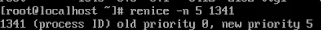
\includegraphics{12.png}
		\item Посмотрите иерархию запущенных процессов: \\
		
\includegraphics{13.png}
		\item Найдите PID корневой оболочки, из которой были запущены процессы dd, и завершите этот процесс: \\
		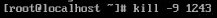
\includegraphics{14.png}
	\end{frame}
\end{enumerate}

\section{Вывод}
\begin{frame}[plain]
	\frametitle{Вывод}
	В ходе выполнения данной работы я получил навыки управления процессами операционной системы.
\end{frame}

\end{document}
